\documentclass[]{article}
\usepackage{lmodern}
\usepackage{amssymb,amsmath}
\usepackage{ifxetex,ifluatex}
\usepackage{fixltx2e} % provides \textsubscript
\ifnum 0\ifxetex 1\fi\ifluatex 1\fi=0 % if pdftex
  \usepackage[T1]{fontenc}
  \usepackage[utf8]{inputenc}
\else % if luatex or xelatex
  \ifxetex
    \usepackage{mathspec}
  \else
    \usepackage{fontspec}
  \fi
  \defaultfontfeatures{Ligatures=TeX,Scale=MatchLowercase}
\fi
% use upquote if available, for straight quotes in verbatim environments
\IfFileExists{upquote.sty}{\usepackage{upquote}}{}
% use microtype if available
\IfFileExists{microtype.sty}{%
\usepackage{microtype}
\UseMicrotypeSet[protrusion]{basicmath} % disable protrusion for tt fonts
}{}
\usepackage[margin=1in]{geometry}
\usepackage{hyperref}
\hypersetup{unicode=true,
            pdftitle={DATA 609 - Homework 7},
            pdfauthor={Joshua Sturm},
            pdfborder={0 0 0},
            breaklinks=true}
\urlstyle{same}  % don't use monospace font for urls
\usepackage{graphicx,grffile}
\makeatletter
\def\maxwidth{\ifdim\Gin@nat@width>\linewidth\linewidth\else\Gin@nat@width\fi}
\def\maxheight{\ifdim\Gin@nat@height>\textheight\textheight\else\Gin@nat@height\fi}
\makeatother
% Scale images if necessary, so that they will not overflow the page
% margins by default, and it is still possible to overwrite the defaults
% using explicit options in \includegraphics[width, height, ...]{}
\setkeys{Gin}{width=\maxwidth,height=\maxheight,keepaspectratio}
\IfFileExists{parskip.sty}{%
\usepackage{parskip}
}{% else
\setlength{\parindent}{0pt}
\setlength{\parskip}{6pt plus 2pt minus 1pt}
}
\setlength{\emergencystretch}{3em}  % prevent overfull lines
\providecommand{\tightlist}{%
  \setlength{\itemsep}{0pt}\setlength{\parskip}{0pt}}
\setcounter{secnumdepth}{0}
% Redefines (sub)paragraphs to behave more like sections
\ifx\paragraph\undefined\else
\let\oldparagraph\paragraph
\renewcommand{\paragraph}[1]{\oldparagraph{#1}\mbox{}}
\fi
\ifx\subparagraph\undefined\else
\let\oldsubparagraph\subparagraph
\renewcommand{\subparagraph}[1]{\oldsubparagraph{#1}\mbox{}}
\fi

%%% Use protect on footnotes to avoid problems with footnotes in titles
\let\rmarkdownfootnote\footnote%
\def\footnote{\protect\rmarkdownfootnote}

%%% Change title format to be more compact
\usepackage{titling}

% Create subtitle command for use in maketitle
\newcommand{\subtitle}[1]{
  \posttitle{
    \begin{center}\large#1\end{center}
    }
}

\setlength{\droptitle}{-2em}

  \title{DATA 609 - Homework 7}
    \pretitle{\vspace{\droptitle}\centering\huge}
  \posttitle{\par}
    \author{Joshua Sturm}
    \preauthor{\centering\large\emph}
  \postauthor{\par}
      \predate{\centering\large\emph}
  \postdate{\par}
    \date{November 13, 2018}


\begin{document}
\maketitle

\hypertarget{chapter-8-problems}{%
\section{Chapter 8 Problems}\label{chapter-8-problems}}

\hypertarget{page-304-exercise-2}{%
\subsection{1 (Page 304, exercise \#2)}\label{page-304-exercise-2}}

The bridges and land masses of a certain city can be modeled with graph
\(G\) in Figure 8.7.

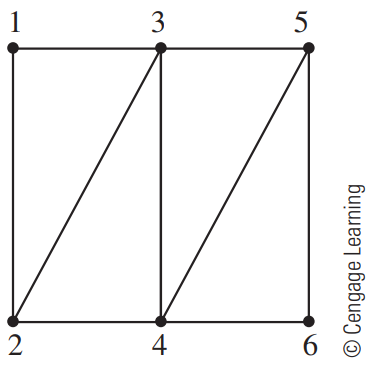
\includegraphics{figure87.png}

\begin{enumerate}
\def\labelenumi{\alph{enumi}.}
\item
  Is \(G\) Eulerian? Why or why not?
\item
  Suppose we relax the requirement of the walk so that the walker need
  not start and end at the same land mass but still must traverse every
  bridge exactly once. Is this type of walk possible in a city modeled
  by the graph in Figure 8.7? If so, how? If not, why not?
\end{enumerate}

\hypertarget{a-solution}{%
\subsubsection{1a Solution}\label{a-solution}}

A graph is Eulerian if: - Every path is reachable and connected - Each
vertex has an even number of connections

Graph \(G\) satisfies the first condition, but fails the second -
vertices 2 and 5 have an odd number of connections (3).

\hypertarget{b-solution}{%
\subsubsection{1b Solution}\label{b-solution}}

Since the graph has two vertices with an odd number of connections, this
would be possible.\\
An example would be:

\[
2 \to 1 \to \to 3 \to 2 \to 4 \to 3 \to 5 \to 4 \to 6 \to 5
\]

\hypertarget{page-307-exercise-1}{%
\subsection{2 (Page 307, exercise \#1)}\label{page-307-exercise-1}}

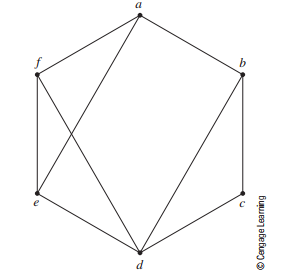
\includegraphics{figure811.png}

\begin{enumerate}
\def\labelenumi{\alph{enumi}.}
\item
  Write down the set of edges \(E(G)\).
\item
  Which edges are incident with vertex \(b\)?
\item
  Which vertices are adjacent to vertex \(c\)?
\item
  Compute \(deg(a)\).
\item
  Compute \(|E(G)|\).
\end{enumerate}

\hypertarget{a-solution-1}{%
\subsubsection{2a Solution}\label{a-solution-1}}

\begin{center}
$E(G) = \{ab, ae, af, bc, bd, cd, de, df, ef\}$.
\end{center}

\hypertarget{b-solution-1}{%
\subsubsection{2b Solution}\label{b-solution-1}}

Edges \(ab, bc, \text{and } bd\).

\hypertarget{c-solution}{%
\subsubsection{2c Solution}\label{c-solution}}

Vertices \(b\) and \(d\) are adjacent to vertex \(c\).

\hypertarget{d-solution}{%
\subsubsection{2d Solution}\label{d-solution}}

The degree of a vertex is the number of incidences between that vertex
and an edge.\\
\(deg(a) = 3\).

\hypertarget{e-solution}{%
\subsubsection{2e Solution}\label{e-solution}}

\(|E(G)|\), or the cardinality of \(E(G)\), is the number of elements in
the set \(E(G)\).\\
From our answer in part 2a, we can see that \(|E(G)| = 9\).


\end{document}
